\documentclass[11pt]{article}
\usepackage[margin=1in]{geometry}                % See geometry.pdf to learn the layout options. There are lots.
\geometry{letterpaper}                   % ... or a4paper or a5paper or ... 
%\geometry{landscape}                % Activate for for rotated page geometry
%\usepackage[parfill]{parskip}    % Activate to begin paragraphs with an empty line rather than an indent
\usepackage{color}
\definecolor{myblue}{rgb}{0.0, 0.0, 0.85}
\usepackage[breaklinks=true, colorlinks=true, linkcolor=red, urlcolor=myblue, citecolor=black]{hyperref}
\urlstyle{rm}
\usepackage{mathptmx}
\usepackage{graphicx}
\usepackage{amssymb}
\usepackage{epstopdf}
\usepackage{sidecap}
\usepackage{authblk}
\usepackage{booktabs}
\usepackage[font=small,labelfont=bf]{caption}
\usepackage{enumitem}
\usepackage{wrapfig}
\DeclareGraphicsRule{.tif}{png}{.png}{`convert #1 `dirname #1`/`basename #1 .tif`.png}
\pagestyle{plain}

\def\bfr{\bf\color{red}}
\def\bfp{\color{magenta}}
\def\geohub{{\tt geohub}}
\def\resp{respectively}
\def\selah{SELAH}
\def\nch{718}
\def\nh{957\pm94}
\def\dh{10\%\pm9\%}
\def\nce{389}
\def\ne{556\pm83}
\def\de{15\%\pm12\%}

\begin{document}
%\maketitle

\begin{center}
	\Large\bf Unsheltered Homelessness in Hollywood Is Down from January 2020 Levels\\
	\vspace{1ex}
	{\normalsize\rm Louis Abramson, PhD, and Brian Kohan 
	for the \href{http://www.hollywood4wrd.live}{\it Hollywood 4WRD Coalition} \\ \today 
	{\bfr \texttt{ -- NOT FOR DISTRIBUTION}}}
\end{center}

\noindent {\bf Summary:} Volunteers surveyed all of Hollywood and East Hollywood on February 25, 
2021, finding the number of people experiencing unsheltered homelessness to have fallen 
by $10\%$ and $15\%$, \resp, compared to the 2020 LAHSA Count. A 30\% drop in individuals on the 
street---as opposed to dwellings---drives this change (Figure \ref{fig:rawCounts}) even as tents doubled in 
28\% of census tracts. This phenomenon could support subjective impressions that the 
state of homelessness has worsened despite a drop in raw numbers. Indeed, COVID-related 
contractions in health, hygiene, and social services, mean that such perceptions may also be accurate. 
Data from the Coordinated Entry System data will reveal if homelessness has declined generally, 
or if government initiatives have reduced Greater Hollywood's share of it.
%, which has lowered the unsheltered population in about a third of census tracts
%Unsheltered living has probably declined quantitatively even if the average occupancy of dwellings has changed. 
%This trend holds in tracts assessed by professionals or volunteers and is larger 
%than counting errors can account for.
% less than a 93\% chance that 
%with at least one preliminary survey suggesting such updates may be modest
%the number of unsheltered people has fallen by at least some amount. %\pm9\% %\pm12\%
%(1/23)
%assuming no changes in average dwelling occupancies, 
%Only seven tracts saw significant increases in raw counts, with makeshift dwellings the only category to increase in both CoCs. 
%All data are available to support future analyses incorporating such information.

\begin{table*}[h!]
\caption{Greater Hollywood 2021 Unsheltered Counts and Population Estimates}
\resizebox{\linewidth}{!}{%
\begin{tabular}{lccccccccc}
\toprule
 & Persons & Cars & Vans & RVs & Tents & Makeshifts & {\bf 2021 Total} & {\bf 2020 Total} & {\bf \% change} \\ \cmidrule{1-10}
{\bf Hollywood} \\ %\cmidrule{1-1}
Counts & 284 & 21 & 30 & 38 & 230 & 116 & {\bf 718} & {\bf 831} & $\bf -14\%$ \\ %831
Inhabitants & 284 (28) & 32 (11) & 54 (14) & 56 (14) & 339 (29) & 195 (24) & {\bf 957 (94)} & {\bf 1058} & $\bf -10\%\,(9\%)$\\% {\bf 1058}(76)
Population share & 29\% (3\%) & 3\% (1\%) & 6\% (1\%) & 6\% (1\%) & 35\% (3\%) & 20\% (3\%) & -- & -- & -- \\ \cmidrule{1-10}
{\bf East Hollywood} \\ %\cmidrule{1-1}
Counts & 118 & 10 & 39 & 16 & 77 & 127 & {\bf 389} & {\bf 469} & $\bf -17\%$ \\
Inhabitants & 118 (19) & 15 (8) & 70 (15) & 24 (9) & 115 (19) & 216 (23) & {\bf 557 (83)} & {\bf 656} & $\bf -15\%\,(12\%)$\\% (60)
Population share & 21\% (3\%) & 3\% (1\%) & 13\% (3\%) & 4\% (2\%) & 20\% (3\%) & 39\% (4\%) & -- & -- &--
\\ \bottomrule
\end{tabular}
}
\caption*{Parentheses denote 90\% uncertainties. Uncertainties larger than estimates 
mean that only upper limits are available.}% No unaccompanied minors or families were observed.}
\label{tbl:summary}% (binomial in the case of the categories)
\end{table*}

\begin{figure*}[h]
	\centering
	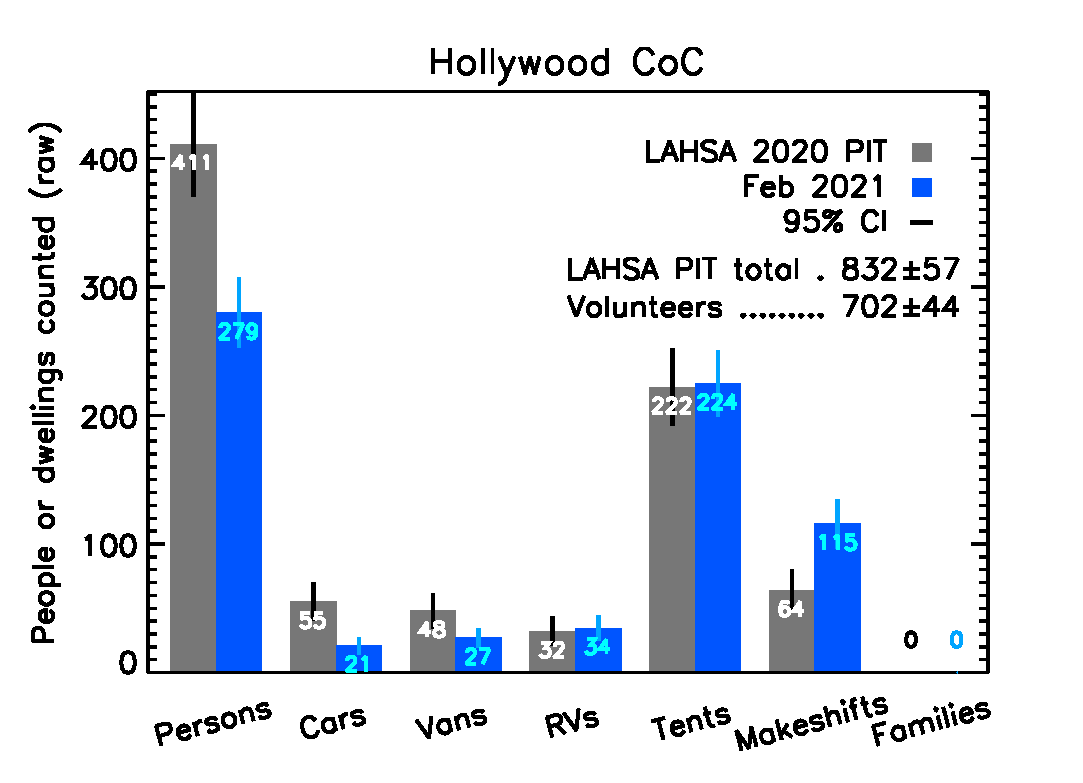
\includegraphics[width = 0.47\textwidth, trim = 1cm 0cm 0cm 0cm]{Hwood2021Bars}
	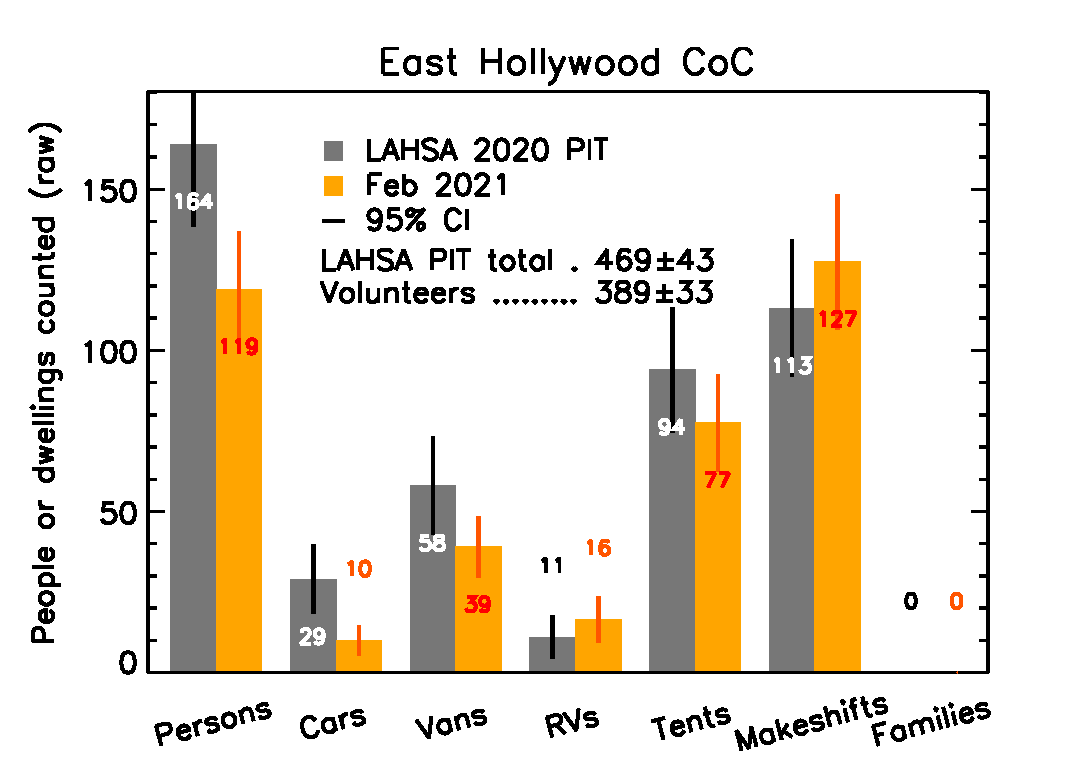
\includegraphics[width = 0.47\textwidth, trim = 0cm 0cm 1cm 0cm]{Eho2021Bars}
	\caption{Raw tallies of unsheltered persons and dwellings in Hollywood and East Hollywood
			(left/right) from the 2020 and 2021 PIT counts (grey/colors). Persons, cars, 
			and vans fell in both communities while RVs and tents stayed statistically flat. 
			Makeshift structures are the only category to show a potential common increase. 
			Overall, we identified 194 fewer people and dwellings compared to 2020,
			with similar 15\% decreases assessed by almost entirely independent teams
			in both communities. ``Persons'' are TAY+Adults.}
	\label{fig:rawCounts}
\end{figure*}

%\begin{figure*}[h!]
%	\centering
%	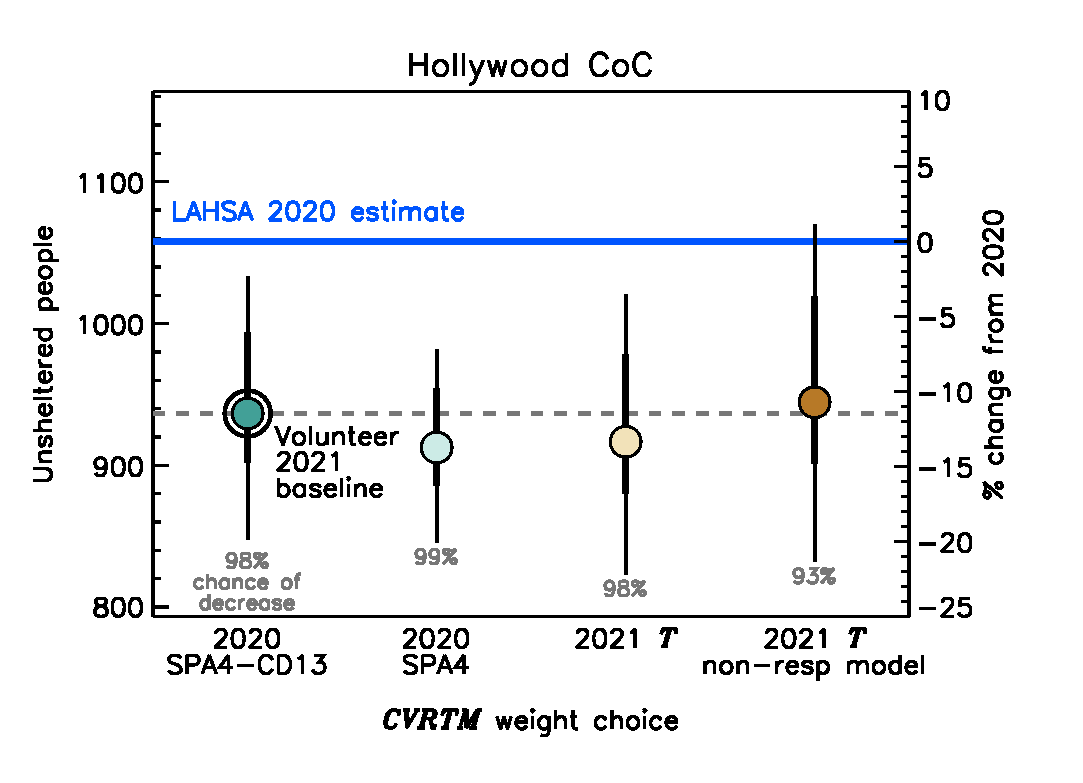
\includegraphics[width = 0.48\textwidth, trim = 0cm 0.5cm 0cm 0cm]{hwoodFinal}
%	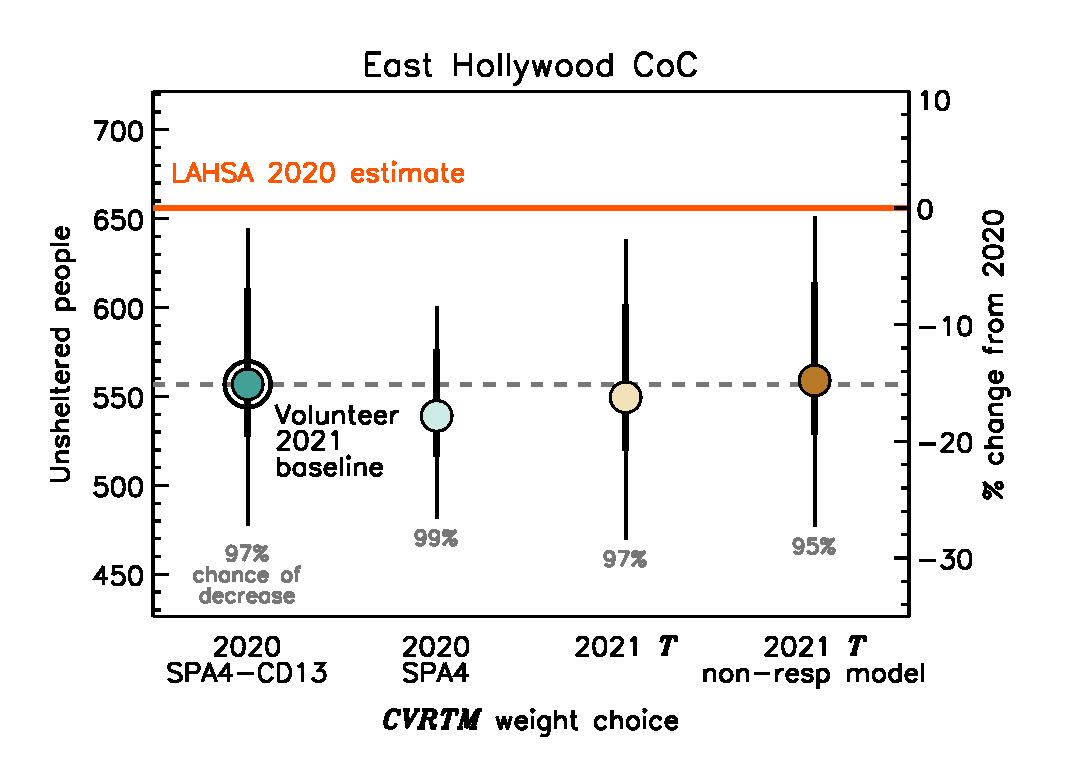
\includegraphics[width = 0.48\textwidth, trim = 0cm 0.5cm 0cm 0cm]{ehoFinal}	
%	\caption{Unsheltered populations in Hollywood (left) and East Hollywood (right) 
%			as functions of CVRTM weights. The baseline estimate uses the same weights as the 
%			2020 LAHSA Community Summaries. Using SPA4 weights or replacing the tent 
%			weight, $T$, with results from a survey conducted in Hollywood yields consistent
%			results. All imply at least a 93\% chance that unsheltered homelessness has fallen
%			by some amount, with likely declines of $12\%\pm9\%$ and $15\%\pm12\%$
%			in Hollywood and East Hollywood, \resp.}
%	\label{fig:wtComp}
%\end{figure*}

%\pagebreak

\noindent {\bf Context:} To compensate for the \href{https://laist.com/latest/post/20201209/LAHSA-cancels-2021-homeless-count-los-angeles-covid-19}
{cancellation} of the 2021 LAHSA Count, nonprofit and volunteer organizations in Hollywood\footnote{
{\it \href{https://thecenterinhollywood.org}
{The Center at Blessed Sacrament}, \href{https://chnc.org}{The Central Hollywood Neighborhood Council}, 
\href{https://www.covenanthouse.org/spring-meal-match?sourceid=2483460&origin=DHQEI2109EZI0N&utm_source=2103marchmealmatchweb&utm_medium=cpc&utm_campaign=FY21MarchMealMatch&utm_content=bsd2103marchmealmatchweb&gclid=CjwKCAiAp4KCBhB6EiwAxRxbpJA2yM7lM2tyAqjVALZgBGvjnhobCJJ0XmuELFDXzM5xxZ0BqyX1ChoCLi0QAvD_BwE}{Covenant House}, 
Hang Out Do Good, \href{https://hollywood4wrd.live}{Hollywood 4WRD}, 
 \href{https://www.myfriendsplace.org/}{My Friend's Place}}, and resident organizers.} conducted a
grassroots enumeration of people experiencing unsheltered homelessness%\begin{figure*}[t]
\begin{wrapfigure}{r}{0.625\linewidth}
	\centering
%	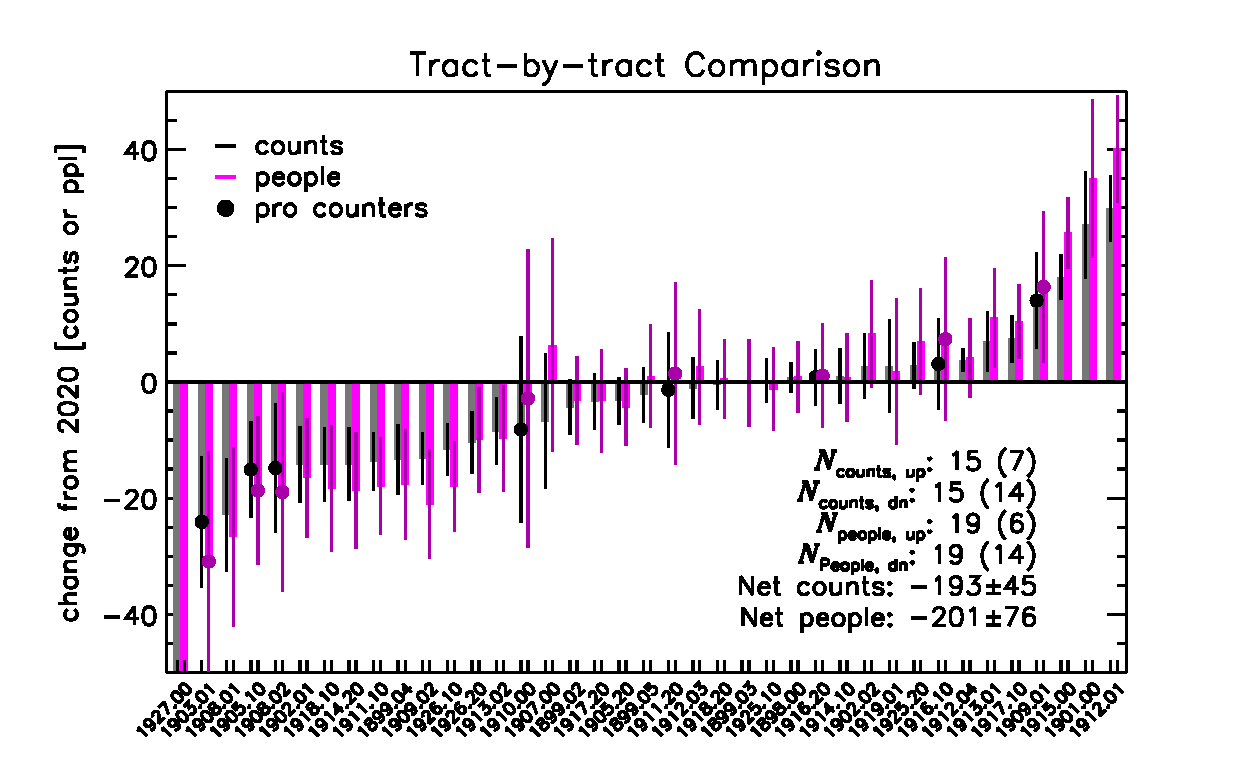
\includegraphics[width = 0.8\textwidth, trim = 0cm 0cm 0cm 0cm]{tractsYrYr}
	\includegraphics[width = \linewidth, trim = 0cm 0.25cm 0cm 0.25cm]{countMap}
	\caption{The count area with census tracts colored by  
			changes in unsheltered population from 2020 (red$+$, blue$-$).
			Hollywood spans Crescent Heights/Franklin to Western/Melrose. East Hollywood 
			spans Hollywood/Western to Hoover/Beverly and saw the largest changes:
			tract 1912.01 rose by 40 people and 1927.00 fell by over 120 people.}
%			Subsequent cross-checks support both tracts' PIT counts.}
	\label{fig:tcomp}
\end{wrapfigure} in all
%\end{figure*} conducted 
census tracts in Hollywood and East Hollywood on Feb.~25, 2021 (Figure \ref{fig:tcomp}).\\

%Nine tracts were counted by professional outreach teams during the %---comprising $\sim$43\% of identified individuals and dwellings---
%day. The remainder were surveyed by car-based volunteer teams starting at 7:00 PM.
%
%Each team surveyed two tracts. To increase accuracy, each tract was surveyed by at 
%least two teams.\\
%Tracts counted by professionals were assessed only once. No 
%volunteers and only one professional team counted tracts in both communities, making the two datasets 
%almost entirely independent.
%and enabling better error estimates
%Year-on-year trends hold across communities and between volunteer- and professional-counted tracts.
%Seven tracts saw significant increases; 14 saw declines. The tracts with the largest increase (1912.01;
%Barnsdall Park) and decrease (1927.00; US 101) are both in East Hollywood.\\
%; volunteer-counted; professional-counted

\noindent {\bf Results:} The population estimates in Table \ref{tbl:summary} %and Figure \ref{fig:wtComp} 
reflect all people, cars, vans, RVs, tents, and makeshift dwellings seen that night, with each
dwelling weighted by its average occupancy. Our baseline result uses the same %quoted in Table \ref{tbl:summary} and shown in teal in Figure \ref{fig:wtComp}
\href{https://www.lahsa.org/documents?id=4635-usc-2018-2020-multipliers-and-estimates-overview}
{SPA4/CD13 weights} as the last official 
\href{https://www.lahsa.org/documents?id=4686-2020-greater-los-angeles-city-community-homelessness-report-service-planning-area-4.pdf}
{LAHSA Community Summaries}. 
%These suggest $\nh$ and $\ne$ people were experiencing unsheltered 
%homelessness, \resp, on 25 Feb.\ (90\% CI). 
Changing weights based on a tent survey or using the last 
\href{https://www.lahsa.org/documents?id=4693-2020-greater-los-angeles-homeless-count-cvrtm-conversion-factors}{SPA4-wide} values has no significant effect.
%\footnote{Those inferences yield $912\pm68$ and $944\pm118$ people
%in Hollywood, and $539\pm59$ and $559\pm87$ in E.~Hollywood, \resp.}  % (Figure \ref{fig:wtComp})
All suggest at least an 89\% chance of a decline compared to 2020. 

Tents would have to shelter $\sim$45\% more people on average now to erase the decline we infer. 
At least since 2018, such a large change has never been seen. The aforementioned tent survey---which 
showed that tent occupancies are similar to 2020---makes it even more unlikely.\footnote{\selah\ 
outreach teams surveyed 47 tents in Hollywood on 28 Feb., finding an average of $1.50\pm0.22$ 
people per tent vs.~LAHSA's 2020 value of $1.48\pm0.11$.}
%however. If the average tent, e.g., holds more people today 
%compared to last year, then part of the inferred population decrease may be an artifact.
%\footnote{The $T$ and $M$ weights are the largest 
%potential errors in this analysis due to the high proportion of people living in tents and makeshift structures. 
%The full 2021 PIT area has not been assessed, but \selah\ outreach teams surveyed 47 tents (38 responses) in 
%Hollywood on 28 Feb., finding a mean occupancy of $T=1.39\pm0.14$ people per tent ($T=1.50\pm0.22$ if 
%non-responses are modeled). $M$ was not estimated, but that $T$ value is consistent with the LAHSA 2020 
%weight of $T=1.48\pm0.11$. We encourage larger efforts to update the CVRTM weights.} 
%the occupancy increases needed to erase our estimated changes are
%substantial. 

Other data suggest that our 2021 enumeration is accurate: (1) 38 duplicate tract measurements 
show that counting errors are consistent with random mistakes, which the analysis accounts for; (2) 
\href{https://hollywoodpartnership.com/}{\it The Hollywood Partnership} found the same result for
a common tract on 19 Feb.; (3) trends in Hollywood and East Hollywood agree despite being counted 
by different teams; (4) a \href{https://selahnch.org}{\selah} recount of a tract in East Hollywood two 
days later agrees with our data. Finally, assuming 80 people may have been at safe parking sites, the 
chance of a decline from 2020 is still 88\%.\\
%\begin{enumerate}
%%	\setlength{\itemsep}{-1ex}
%	\item Our 38 duplicate tract measurements suggest counting uncertainties are consistent with random 
%		errors, which the analysis accounts for.
%%		\begin{itemize}
%%			\item Tract 1901.00---the only outlier in the above comparisons---was independently recounted 
%%				14 hours after the PIT count with results consistent with the average of the volunteer teams' 
%%				results.
%%			\item Tract 1912.01---largest increase---was independently recounted on 27 Feb.\ circa 
%%				12:00 PM with results similarly consistent with the PIT teams' assessments.
%%			\item Tract 1927.00---largest decrease---was independently recounted on 4 March at 
%%				8:30 AM with results lower than the PIT's assessment. This especially dense tract was originally 
%%				surveyed on foot by outreach professionals, however, with the recount was performed by a car-based
%%				volunteer. The cross-check therefore suggests only that the PIT data are not biased in ways that
%%				would induce an artificial year-on-dear decline.				
%%		\end{itemize}
%	\item A census by \href{https://hollywoodpartnership.com/}{\it The Hollywood Partnership} 
%		from 19 Feb.\ agrees with our data in a common tract.% and an independent 
%%		recount of that entire geography performed 28 Feb.% also show a decline from past values and 
%	\item Trends are common to Hollywood and East Hollywood despite being counted by different teams.%in tracts counted by volunteers and professionals
%	% (reduced individuals, flat
%%		or marginally higher dwelling counts).
%%	\item Tracts monitored by \selah\ since May 2020 show similar declines to that implied by our data. 
%%		One of these tracts is 1912.01 in East Hollywood, whose 27 Feb.\ \selah\ estimate  agrees with our 
%%		PIT value.% in unsheltered homelessness.
%	\item A recount of one tract in East Hollywood by
%		\href{https://selahnch.org}{\selah} on 27 Feb.\ agrees with our data.% 1912.01
%\end{enumerate}

%		   P	C     V	    R	 T     M
%1901.00 -- 50    8    5.5   1     6      4 -- 2021, raw
%1901.00 -- 36    4     6     0     8      2 -- 26 Feb ABRAMSON 9.00 AM
%
%1927.00 -- 48    1      5     0    53    70 -- 2020, raw
%1927.00 -- 20    0     0     7     6     54 -- 2021, raw
%1927.00 -- 15     0     9     5    14    21 -- 4 Mar 2021 ABRAMSON 8.45 AM
%
%1912.01 --  18.5  0.5  3.5  1.5  5.5  12 -- 2021, raw
%1912.01 --  21     0      4     1     8      6  -- 27 Feb ABRAMSON 12.15 PM
%
%1902.02 -- 9      --     --     --     8   5.5 -- 2021, raw
%1902.02 -- 9      --     --     --    17    --  -- BID 2/19

% 1907.00 is also interesting in that total population stayed nearly the same but identified
% individuals and dwellings basically swapped: IND 73->38; CVRTM 31->70. This has a big impact
% on people's perceptions, and it's in a very high-traffic part of the community.

%The pro/vol trends are consistent everywhere except tract 1927.00, 
%			where pro counts dropped significantly more for both individuals and dwellings (esp.\ 
%			tents). 1927.00 comprises 22\% of total counts in East Hollywood. Unsheltered 
%			homelessness in that CoC was flat or rose slightly outside of that tract.}
%{\bfr 1927.00 is the tract with the PATH Madison PSH. Phase II opened in Jan 2020---leasing began May 
%2020---and is 120 units, some of which were filled from nearby folks but I dunno how many. LEA recounted 
%this tract 4 March at $\sim$9:00 AM and found 94 total population vs.\ pro's 129. Only place where
%LEA counted more objects was vans. Adding that to the pro total adds 16 people (9 vans).

% All of the above suggests that our results are reliable.\\
%Assumes equal mix of cars + vans.
%From Starkey: Hwood = 25, Eho = 10, EchoPk = 14; total = 49; total CD13 = 59 but I think it's reasonable
%to truncate at Echo Pk. It's 90% if you include all 59 spaces.

\noindent {\bf Comments:} The drop we find mainly reflects $\sim$30\% fewer adults seen on the 
street. This fact has caused the total number of unsheltered people to shrink even as tents more than
doubled in 28\% of tracts. Government initiatives to stop evictions and move people indoors and may be 
responsible. If \href{https://www.lahsa.org/documents?id=4672-2020-homeless-count-council-district-13}{CD13's} 6.5\% share of \href{https://www.lahsa.org/documents?id=4585-2020-greater-los-angeles-homeless-count-los-angeles-continuum-of-care-coc-}{LA County's unsheltered seniors} is an indication, 100 
Greater Hollywood residents may have occupied Project Roomkey's 
\href{https://projectroomkeytracker.com/}{1608 active rooms} on the night of the count---enough to
account for about half the inferred change. The new Riverside \href{https://www.lamayor.org/ABridgeHome}
{\it A Bridge Home} and 120 PATH supportive housing units may also have contributed.
%The latter are located in tract 1927.00. While all of those units did not go to local residents, any that did would help
%drive that tract's large observed decrease. 
Coordinated Entry System data will show if the above scenarios are true.
%1927.00 is actually in the catchment of 3 ABHs that were either new or expanded between PIT counts. 
%Lodi, however, did not fill its new beds, and Lafayette doesn't cover the whole tract, so we won't speculate.
%Nevertheless, technically, even at 50\% decompression, residents of 1927.00 may have been eligible 
%for any of 89 new ABH beds. It's also on the CoC boundary.

If there are fewer people on the street, however, their quality of life is worse. 
COVID has restricted or eliminated access to restaurant bathrooms, libraries 
(\href{https://www.lapl.org/homeless-resources/the-source}{\it The Source}), DPSS 
(EBT, Medi-Cal), DMV (IDs), and DMH facilities. Physical limits on client access at 
hospitals has also kept caseworkers from managing successful discharges. These harms 
are reflected by a 25\% increase in 
\href{https://www.latimes.com/california/story/2021-01-07/the-powerful-synthetic-opioid-fentanyl-is-behind-rising-deaths-in-the-homeless-population}{overdose deaths} and made more visible by \href{https://clkrep.lacity.org/onlinedocs/2020/20-0147_misc_3-17-20_p.pdf}{suspended}
tent folding and sanitation practices as tents increased in many places. 
Of course, the $\sim$10\% decline we infer does not bode well for the period \href{https://www.latimes.com/california/story/2021-01-12/new-report-foresees-tens-of-thousands-losing-homes-by-2023}
{after the eviction moratoriums end}.

If our data support the effectiveness of programs aimed at reducing street homelessness, 
they do {\it not} suggest that the state of homelessness has improved. In the fight to rebuild lives---as well 
as build homes---that fact must remain paramount.

%\clearpage

%HOLLYWOOD -- Zero delta requires CVRTM mean occupancies of:\\
% - 5.00 ppl/car (from 1.51)\\
% - 5.00 ppl/van (from 1.77)\\
% - 4.95 ppl/RV (from 1.42)\\
% - 2.03 ppl/tent (from 1.48)\\
% - 2.73 ppl/mkshft (from 1.68)\\
%
%EAST HOLLYWOOD -- Zero delta requires CVRTM mean occupancies of:\\
% - 5.00 ppl/car (from 1.51)\\
% - 4.33 ppl/van (from 1.77)\\
% - 5.00 ppl/RV (from 1.42)\\
% - 2.78 ppl/tent (from 1.48)\\
% - 2.45 ppl/mkshft (from 1.68)


% ------ SUMMARY for HWOOD ------ 
%
%Total People (90%CI) .   936+/-92
%Fraction vs. last yr .   0.89+/-0.09
%Total counts..........   702
% > Adults    : 277 (39%), 277, (29%)
% > TAY       :   2 ( 0%),   2, ( 0%)
% > Minors    :   0 ( 0%),   0, ( 0%)
% > Cars      :  21 ( 2%),  31, ( 3%)
% > Vans      :  27 ( 3%),  47, ( 5%)
% > RVs       :  34 ( 4%),  49, ( 5%)
% > Tents     : 224 (31%), 330, (35%)
% > Makeshifts: 115 (16%), 193, (20%)
% > Families  :   0 ( 0%),   0, ( 0%)
%% Compiled module: MINMAX.
%Min/max ppl/tract ..... 0, 169
%Min/max counts/tract .. 0, 123
%
% ------ SUMMARY for EHO ------ 
%
%Total People (90%CI) .   556+/-83
%Fraction vs. last yr .   0.85+/-0.13
%Total counts..........   389
% > Adults    : 114 (29%), 114, (20%)
% > TAY       :   4 ( 1%),   4, ( 0%)
% > Minors    :   0 ( 0%),   0, ( 0%)
% > Cars      :  10 ( 2%),  14, ( 2%)
% > Vans      :  39 (10%),  68, (12%)
% > RVs       :  16 ( 4%),  23, ( 4%)
% > Tents     :  77 (19%), 114, (20%)
% > Makeshifts: 127 (32%), 214, (38%)
% > Families  :   0 ( 0%),   0, ( 0%)
%Min/max ppl/tract ..... 6, 129
%Min/max counts/tract .. 5, 87

%%%%%%%
%%%%%%%
%%%%%%%

%\begin{center}
%-- notes --
%\end{center}

%{\bfr VISUAL DISPLAY VS NUMBERS -- SEE PEOPLE WHO'VE MOVED TO VALLEY RETURNING 
%TO HOLLYWOOD FOR SERVICES DURING THE DAY.}
%
% {\bfr Five ABH's cover Greater Hollywood,
%three have catchment areas covering 1927.00. Their net addition is 33 beds, total, but 89 in that tract (whose
%net gain is eroded by losses of preexisting beds from Schrader and Garnder in the west).}

%DPSS closed; phone system with long waits req'd to replace EBT. If you don't have a phone your stuck.

%Libraries are closed, and therefore {\it The Source} service connection events. 
%Daytime charity resources and some parks are closed, resulting in more exposure to the weather and less food.

%Med-Cal not accessible via DPSS. Enrolling in health insurance requires similar phone calls and that a state 
%ID be uploaded (previously not required). Lacking insurance affects likelihood and length of admission to hospital. 
%Discharges requiring skilled or recuperative care placements are even more difficult.

%DMV is by appointment only and appointments are made online.

%DMH clinic services done via telehealth, leaving homeless clients hanging. One FSP has abandoned all field work due to COVID. 
%Clients in crisis needing evaluations redirected to hospitals.

%Hospitals, IMD's step down facilities and SNF's do not allow visitors, limiting the ability of case managers to negotiate 
%with clients and social workers to ensure successful discharges. Consent forms for sharing info cannot be signed by patients 
%due to lack of access.
%
%Homeless people have gotten sicker while hospitals and LAFD have become overburdened dealing with COVID fallout, 
%resulting in less access to emergency care.

%{\bfr KANAGI: ``we've seen a visual drop; dunno where they went but...'' On 2/18 they found 136 
%total tents in the BID vs our 127 (I haven't vetted the rest of the lines; that's just 12\# hot so w/e). (Also 99
%ppl compared to our 89, and 7 vehicles to our 10 and we weren't tracking those as hard as tents.) 
%On the 5th, they counted 163. That's a 17\% decline in 2 weeks, a little more that what we've seen year on year.
%Suggests maybe something happened in early Feb.? -- 3/2 @ 9:55 AM. The tent+mkshft count in 1902.02 is also 
%right on..}

%Only seven tracts saw significant increases in raw counts, with makeshift dwellings the only category to increase in both CoCs. 

%Cars and vans are hard to count, but there's no evidence of a bias. I repeated the most deviant tract the next day, 
%and another tract the day after that. In the latter case, both of my estimates were 0.5 units off the mean, in the 
%former, vans were at that level and I counted fewer cars. Brian and I also recovered a consistent amount of vehicles 
%with the BID (10 vs. their 6 separated by 20+ days). The rest of the tracts show a mean inter-counter bias of 0.6 
%cars (0.4 std.~err) and 1.24 ($0.76\sigma$) vans across all tracts, which should be accounted for in the MC.

% Pro teams counted areas comprising $\sim$43\% of the total raw counts. Three out of these 4 tracts 
% were counted by Covenant House teams, but 1927.00 has the largest drop of any tract and is Elyse 
% from The Center. That tract is basically responsible for the entire decline in East Hollywood, and most 
% of that is in reduced tents, so we should 	talk to these teams.

%%%%%%%
%%%%%%%
%%%%%%%

\end{document}  